% ICIEV / IJCVSP review manuscript audited against the updated notebook.
% Legacy unused PSTricks dependency: use color-only fallback when unavailable.
\IfFileExists{pstcol.sty}{}{%
  \RequirePackage{xcolor}
  \expandafter\def\csname ver@pstcol.sty\endcsname{2026/10/10 color-only compatibility fallback}
}
\documentclass[doublecolumn]{ijcvsplatex}

\usepackage[T1]{fontenc}
\usepackage{lmodern}
\usepackage{microtype}
\usepackage{graphicx}
\usepackage{tikz}
\usetikzlibrary{arrows.meta,positioning}
\usepackage{amsmath}
\usepackage{amssymb}
\usepackage{etoolbox}
\usepackage{booktabs}
\usepackage{array}
\usepackage{tabularx}
\usepackage{url}
\urlstyle{sf}
\usepackage[hidelinks,bookmarks=false]{hyperref}

\newcolumntype{P}[1]{>{\raggedright\arraybackslash}p{#1}}

% Suppress the template's example acceptance, publication dates, and volume.
\makeatletter
\def\@received{}
\def\@revised{}
\def\@accepted{}
\def\@online{}
\def\@vol{}
\patchcmd{\MaketitleBox}{Article History:}{}{}{}
\makeatother
\interdisplaylinepenalty=2500
\emergencystretch=2em

\begin{document}
\begin{frontmatter}

\title{\LARGE LightBanglaHC: Evaluation Validity, Inference Reconstruction, and Accounting Boundaries in Harmful-Content Classification}

% Anonymous review: all three author details are entered in CMT.
% For the final author version, complete author-details.tex then uncomment:
% % Inactive during double-blind review. Do not input this file for initial submission.
% Confirmed first author: Shamim Hasan.
% Two additional authors: exact names not supplied.
% Affiliations, emails, corresponding author and author approvals not supplied.
% Enter all three authors accurately in CMT before initial submission.
% Add actual template author/address commands only after acceptance and confirmation.


\begin{abstract}
Evaluating the efficiency of a harmful content classifier requires separating a small prediction component from the complete pipeline that produces its inputs. We study this separation through a retrospective audit of the updated LightBanglaHC notebook for the HerWILL AI for Digital Safety Datathon 2026. Its recorded three-fold run uses 47,817 labeled training examples, 11,955 unlabeled test rows, four TF-IDF branches with 230,105 combined features, and 20 additional numerical features for LightGBM. Six base candidates and a logistic regression stacker feed a selected weighted ensemble with pooled out-of-fold macro-F1 0.5314, versus 0.5221 for the strongest base candidate. This gap is descriptive and does not establish superior generalization. Globally fitted transformations and class weights, nonnested meta validation, early stopping, outcome-derived ensemble weights, and threshold and candidate selection connect fitting to the reported scores. Source analysis shows why excluding each row from its own base fit does not isolate the complete procedure. The zero-parameter identity module is profiled separately and is absent from the selected prediction path. The exported value 0.183 is derived from a target score rather than a parameter measurement. Six base logistic regression fits alone imply 4,141,908 coefficients and intercepts under the recorded dimensions. We distinguish source observations, recorded outputs, direct data checks, arithmetic reconstruction, and prospective proposals. \par\medskip\noindent\textbf{Contribution of the Paper:} The study provides an inspectable case of alignment among inference, evaluation, and accounting, with a corrected protocol for evaluation and resource reporting; it introduces no new classification algorithm or demonstrated deployment advantage.
\end{abstract}
\begin{keyword}
Harmful-content classification \sep Evaluation validity \sep Stacked
generalization \sep Accounting boundaries \sep Reproducibility.
\end{keyword}
\end{frontmatter}

\section{Introduction}
\label{sec:introduction}

A harmful content classifier's reported accuracy and efficiency are interpretable only when they refer to a specified prediction procedure. In sparse ensembles, predictions can depend on fitted representations, calibrated base estimators, and a second-stage head. Counting the head alone does not describe the system that produces its inputs~\cite{schwartz2020greenai}.

We distinguish three objects: the \emph{inference object}, which maps raw text to predictions; the \emph{evaluation object}, which includes fitting, validation, and selection; and the \emph{accounting object}, which defines the artifacts and computation included in a resource claim. Stacking~\cite{wolpert1992stacked} makes their relationship consequential: excluding a row from its own base fit does not necessarily isolate the full procedure when meta training features depend on meta validation labels. Global preprocessing and repeated selection create additional dependencies~\cite{varma2006bias,cawley2010overfitting,kapoor2023leakage}.

We examine one recorded LightBanglaHC implementation from the HerWILL AI for Digital Safety Datathon 2026. The updated notebook, retained outputs, competition description, and raw CSVs permit source inspection, data checks, inference reconstruction, and arithmetic accounting. Row level OOF predictions and fitted artifacts remain unavailable, so we neither rerun training nor authenticate recorded predictions by replay. Documentation describes a mixed Bangla, English, and Banglish corpus; preprocessing alone would not establish this scope.

The contribution is an inspectable audit linking the three objects within one artifact, followed by a corrected prospective protocol. It is not a new algorithm, a demonstration of predictive superiority, or a measured deployment advantage. Section~\ref{sec:design} defines the evidence categories and verification limits used throughout.

\section{Related Work}
\label{sec:related}

\subsection{Harmful Content Constructs and Bangla Resources}
\label{sec:rw-constructs}
Hate speech and offensive language require distinct annotation decisions~\cite{davidson2017automated}; multi-aspect schemes also document dimensions such as hostility and targets~\cite{ousidhoum2019multilingual}. Functional tests expose weaknesses that aggregate scores can obscure, including responses to negation and counter speech~\cite{rottger2021hatecheck}. Bias analysis further requires stating which harms matter and to whom~\cite{blodgett2020language}. Without an annotation manual, LightBanglaHC's "subtle" class cannot be interpreted as a validated category of sarcasm or implicitness.

\label{sec:rw-bangla}
BD-SHS provides a Bangla hate speech resource with hierarchical annotation~\cite{romim2022bdshs}, while BanglaBERT provides pretrained language representations and Bangla understanding benchmarks~\cite{bhattacharjee2022banglabert}. These works supply context rather than directly comparable scores: no verified link connects their data or label definitions to the HerWILL corpus. Data statements document curation and population scope~\cite{bender2018datastatements}, information only partly available for this audit.

\subsection{Stacking, Calibration, and Evaluation}
\label{sec:rw-stacking}
Stacked generalization trains a combiner from base predictions~\cite{wolpert1992stacked}. Complement Naive Bayes is a distinct estimator designed to address assumptions of conventional Naive Bayes text classification~\cite{rennie2003tackling}. Calibration adds fitted state to the probability-generation path~\cite{niculescumizil2005probabilities}; library versions therefore matter when reconstructing both predictions and retained estimators~\cite{pedregosa2011scikit}.

\label{sec:rw-eval}
Model selection can bias an estimate when the same information supports tuning and assessment~\cite{varma2006bias,cawley2010overfitting}. Leakage includes dependencies introduced outside the final estimator fit~\cite{kapoor2023leakage}. Overlapping cross-validation folds require care in uncertainty estimation~\cite{bengio2004variance}, and paired comparisons require predictions and a test appropriate to the experimental design~\cite{dror2018significance}. Probability calibration also requires evaluation separate from classification accuracy~\cite{vaicenavicius2019calibration}. These principles motivate tracing the complete ancestry of meta features rather than accepting an OOF label as proof of isolation.

\subsection{Resource Reporting and Contribution}
\label{sec:rw-accounting}
Green AI motivates reporting computational cost together with predictive performance~\cite{schwartz2020greenai}. Energy reporting~\cite{henderson2020systematic}, reproducibility programs~\cite{pineau2021reproducibility}, and model cards~\cite{mitchell2019modelcards} distinguish resource measurements, replay evidence, and intended use.

\label{sec:rw-summary}
The present study applies established evaluation and reporting principles to one recorded harmful content pipeline. Its specific contribution is the joint reconstruction of prediction dependencies, selection exposure, and the boundary behind zero and fractional parameter claims. We do not claim that leakage or incomplete accounting is a newly discovered general problem, or that this selective review establishes an absence of prior audits.

\section{Study Design, Evidence, and Dataset Scope}
\label{sec:design}

\subsection{Design and Audit Method}
The unit of analysis is the relationship among the implementation, retained outputs, and supported claims. We trace invoked fitting, prediction, selection, profiling, and saving operations through their inputs; comments do not establish execution. We inspect the supplied updated notebook and check raw CSV shapes, labels, identifiers, and exact text duplication. We also reconstruct metrics from its embedded confusion figure. These checks substantiate source structure and internal consistency, not authenticated historical execution.

Each claim has an evidence type: S (source observation), R (recorded output), D (direct CSV check), A (arithmetic reconstruction), X (unverified external quantity), or P (prospective proposal). An unperformed experiment is stated as such. No training, calibration, threshold search, or fresh prediction replay was performed by this audit. Source locations and full file digests are provided in the accompanying artifact ledger rather than abbreviated identities that cannot uniquely match a file.

\subsection{Available Artifacts and Version Boundaries}
The updated notebook contains one code cell, 971 source lines, execution count one, two output streams, and one embedded figure. Its metadata dates execution to 20 April 2026, with a recorded duration of 9,142.89 seconds. This metadata is a retained record, not an independently authenticated timestamp. The notebook's output says \texttt{Device: cuda}, whereas its Kaggle metadata sets GPU enablement false. Python metadata lists 3.12.12; package versions and actual device identity are not logged.

This notebook is distinct from earlier materials. A prior manuscript reports a five-fold, 39-parameter TinyLinear path and macro-F1 0.5295. Another supplied notebook reports four classes, 54,817 training rows, 14,955 test rows, a 68-parameter head, and SVC selection. Neither supplies the execution record analyzed here. The updated source instead selects a weighted ensemble over six base candidates and one stacker. Its figures and numbers replace earlier-run claims in this paper; the historical files are preserved separately for provenance.

The 2026 dataset ZIP contains the three-class CSVs. Separately supplied loose CSVs contain the larger four-class version, with 5,630 repeated training identifiers and 620 repeated test identifiers beyond their first occurrence (D). The smaller files are exact trailing tabular subsets of the larger ones. This relationship does not make the larger version interchangeable with the competition's three-class task. We use only the three-class archive for direct dataset checks.

\subsection{Task and Checked Corpus}
The supplied competition description maps 0 to Explicitly Toxic/Hateful, 1 to Subtly Toxic, and 2 to Non-toxic/Neutral. Training columns are \texttt{id}, \texttt{text}, and \texttt{y}; test columns are \texttt{id} and \texttt{text}. Shapes are (47,817, 3) and (11,955, 2) before processed columns are added (D), totaling 59,772 rows. Table~\ref{tab:supports} reports the class supports, which also match the updated notebook's printed counts.

\begin{table}[t]
\small\centering
\caption{Directly checked supports (D); proportions and globally balanced class weights (A). The source computes weights before splitting (S).}
\label{tab:supports}
\begin{tabular}{lrrr}
\toprule
Class & Support & Proportion (\%) & Weight \\
\midrule
Explicit & 23,756 & 49.681 & 0.670946 \\
Subtle & 18,163 & 37.984 & 0.877553 \\
Neutral & 5,898 & 12.335 & 2.702442 \\
\midrule
Total & 47,817 & 100.000 & \\
\bottomrule
\end{tabular}
\end{table}

The source uses $w_c=n/(3n_c)$ for LR, SVC, SGD, Meta-LR, and LightGBM sample weights. CNB has no explicit class weight argument. Since weights depend on every training label, they also depend on each fold subsequently used for assessment. The test rows have no labels and support no accuracy measurement.

Exact raw string checks find 621 repeated training rows and 54 repeated test rows beyond first occurrences, and 254 distinct texts shared between train and test (D). Identifiers are unique within each three-class file and disjoint between its train and test sets. Text overlap and identifier uniqueness are different properties. We neither estimate the effect of duplication nor perform a near-duplicate, shared-author, or thread analysis.

\subsection{Documentation and Population Scope}
The supplied description presents the corpus as manually annotated Bangla, English, and Banglish social media text from publicly accessible sources, including comments, captions, headlines, and status updates. It emphasizes sarcasm, coded language, code mixing, and noisy text. These are documentation claims, not measured language proportions or verified annotation agreement. The accompanying details document lists CC BY-NC-ND 4.0. It does not supply a complete annotation manual, collection dates, consent records, or annotator-welfare documentation.

The intended label meanings are therefore available, but construct validation remains incomplete. A class called Subtly Toxic does not by itself validate sarcasm detection, and a script indicator is not a language-identification evaluation. The audit makes no claim that the original release lacked documentation; it describes what was supplied for inspection.

\section{Updated LightBanglaHC Pipeline}
\label{sec:pipeline}

\subsection{Cleaning, Signals, and Numerical Features}
Let $x$ be the original string after missing-value handling. The combined processed text is
\begin{equation}
s(x)=C(x)\,\|\,\texttt{SSEP}\,\|\,H(x),
\end{equation}
where $C$ cleans text and $H$ produces signal tokens from the original input. The cleaner applies NFKC normalization, lowercasing, URL and mention substitutions, hashtag-marker removal, emoji substitution, repeated-letter reduction, repeated-punctuation markers, and whitespace compression (S). Signals retain access to original capitalization and punctuation rather than only the cleaned string.

The explicit lexical union contains 21 Bangla, 23 transliterated, and 29 English entries, totaling 73 distinct strings; the subtle inventory contains 25 entries (S). Lexical detection tests substring presence, counting each distinct entry at most once per text, rather than counting every occurrence. Signals include capped repetition of explicit, subtle, sarcasm, threat, identity-related, script, capitalization, punctuation, length, and neutral markers. The string ``this is a salad'' activates the substring \texttt{sala}; this match records a lexical condition rather than intent.

Twenty numerical features are generated without fitted scaling. They cover length, word count, lexical diversity, punctuation, emoji runs, Bangla regex runs, script indicators, capitalization, lexical hits, pattern flags, a combined cue count, and short/long indicators. One feature divides the number of Bangla regex runs by character length; it is not a measured fraction of Bangla characters. Numerical features are supplied to LightGBM only. A marker named for hate or neutrality is a code identifier, not a validated social construct.

\subsection{Four Globally Fitted Sparse Branches}
Table~\ref{tab:features} lists the feature branches and recorded widths. All use sublinear term frequency and are fitted on all processed training texts before the three-fold split. Test texts are transformed, not fitted on (S). Under the documented default interpretation of omitted smoothed-IDF and normalization options, a branch computes
\begin{equation}
\begin{aligned}
u_{ij}&=(1+\ln t_{ij})\left[1+\ln\frac{n+1}{\mathrm{df}_j+1}\right],\quad t_{ij}>0,\\
\phi(x_i)&=u_i/\|u_i\|_2,
\end{aligned}
\end{equation}
with $u_{ij}=0$ otherwise. Historical package versions and fitted arrays are absent; current documentation is not evidence of the original runtime.\footnote{Consulted API: \url{https://scikit-learn.org/1.5/modules/generated/sklearn.feature_extraction.text.TfidfVectorizer.html}.}

\begin{table*}[t]
\small\centering
\caption{Source settings (S) and realized widths printed by the updated notebook (R). Numerical features are appended only for LightGBM.}
\label{tab:features}
\setlength{\tabcolsep}{4pt}
\begin{tabular}{llllrr}
\toprule
Branch & Input & Analyzer & Grams / document frequency & Cap & Width \\
\midrule
Word & $s(x)$ & Word; non-whitespace tokens & 1--3; min 1, max 0.98 & 100,000 & 100,000 \\
Character & $s(x)$ & \texttt{char\_wb} & 2--5; min 2 & 80,000 & 80,000 \\
Clean character & $C(x)$ & \texttt{char} & 1--4; min 2 & 50,000 & 50,000 \\
Signal & $H(x)$ & Word; non-whitespace tokens & 1--2; min 1 & 10,000 & 105 \\
\midrule
Combined TF-IDF & & & & 240,000 & 230,105 \\
LightGBM input & TF-IDF + numerical & & 20 fixed numerical features & & 230,125 \\
\bottomrule
\end{tabular}
\end{table*}

CNB receives both character branches, totaling 130,000 columns. LR, SVC, and SGD receive the 230,105-column TF-IDF matrix. LightGBM receives that matrix plus 20 numerical columns. The global map $\phi$ exposes validation covariates to vocabulary construction, document-frequency filtering, feature caps, and IDF. A later estimator fit that excludes a row cannot undo this earlier representation fitting.

\subsection{Base Candidates and Stacker}
The source forms shuffled stratified three-fold splits with seed 42. Six base candidates are trained: two LR configurations, calibrated SVC, calibrated CNB, calibrated SGD, and LightGBM~\cite{ke2017lightgbm}. Table~\ref{tab:configs} gives explicit settings. The two LR candidates share an estimator family; six candidates do not imply six distinct algorithmic families.

\begin{table*}[t]
\small\centering
\caption{Invoked settings in the updated source (S). Unspecified settings depend on the unrecorded historical library versions.}
\label{tab:configs}
\begin{tabularx}{\textwidth}{llX}
\toprule
Candidate & Input & Explicit configuration \\
\midrule
LR\_C8, LR\_C3 & TF-IDF & $C=8$ or 3; saga; multinomial; max. 2,000 iterations; tolerance $10^{-3}$; global class weights; seed 42. \\
SVC & TF-IDF & LinearSVC, $C=0.5$; max. 3,000 iterations; global class weights; seed 42; isotonic calibration, CV $=2$. \\
CNB & Two character branches & $\alpha=0.05$; \texttt{norm=True}; isotonic calibration, CV $=2$; no explicit class weights. \\
SGD & TF-IDF & Modified Huber; $\alpha=10^{-4}$; max. 200 iterations; global class weights; seed 42; isotonic calibration, CV $=2$. \\
LightGBM & TF-IDF + 20 numerical & Multiclass log loss; 63 leaves; rate 0.1; feature fraction 0.7; bagging fraction 0.8, frequency 5; min. child samples 20; $L_1=0.1$, $L_2=0.5$; \texttt{is\_unbalance=True}; global sample weights; seed 42; max. 1,000 rounds; early-stopping patience 80. \\
Meta-LR & 18 probabilities & $C=10$; max. 500 iterations; multinomial; global class weights; seed 42; solver not overridden. \\
\bottomrule
\end{tabularx}
\end{table*}

Calibration adds fitted state to the probability path~\cite{niculescumizil2005probabilities}. SVC and SGD use global class weights, whereas CNB does not. Their calibration fits remain inside each base fitting subset but share globally fitted features. No proper-score or reliability diagnostic evaluates these probabilities~\cite{vaicenavicius2019calibration}. LightGBM's stopping criterion uses the same validation fold later scored for macro-F1; log loss and macro-F1 are different objectives.

\subsection{OOF Features and Selected Test Predictor}
Let $V_1,V_2,V_3$ partition $I=\{1,\ldots,n\}$, and let $f(i)$ identify row $i$'s fold. For base candidate $b$, let $h_b^{(-f)}$ be its probability-producing fit excluding $V_f$, with calibration or early stopping as specified. Training and test meta features differ:
\begin{equation}
\begin{aligned}
z_i&=\left[h_b^{(-f(i))}(\phi(x_i))\right]_{b=1}^{6}\in\mathbb{R}^{18},\\
\bar z(x)&=\left[\frac{1}{3}\sum_{f=1}^{3}h_b^{(-f)}(\phi(x))\right]_{b=1}^{6}.
\end{aligned}
\end{equation}
LightGBM additionally receives the numerical features, suppressed in this notation for readability. The notation excludes a fold from its base estimator fit, not from global preprocessing, class weights, or LightGBM stopping selection.

Three Meta-LR fits are trained from the single global OOF feature matrix using the same split scheme. Their test probabilities are averaged. The selected final predictor combines six averaged base outputs and the averaged Meta-LR output, so Meta-LR is an active component rather than merely an alternative candidate. If $F_j$ is candidate $j$'s pooled OOF macro-F1 and $p_j(x)$ its test probability vector, then
\begin{equation}
\alpha_j=\frac{F_j^2}{\sum_{k=1}^{7}F_k^2},\qquad
\hat y(x)=\arg\max_c\sum_{j=1}^{7}\alpha_j p_j(x)_c.
\label{eq:ensemble}
\end{equation}
The weights are learned from labeled evaluation outcomes. ``Weighted'' therefore does not mean a prespecified, label-independent average. Figure~\ref{fig:pipeline} separates this prediction path from the independent profiling operation.

\begin{figure*}[t]
\centering
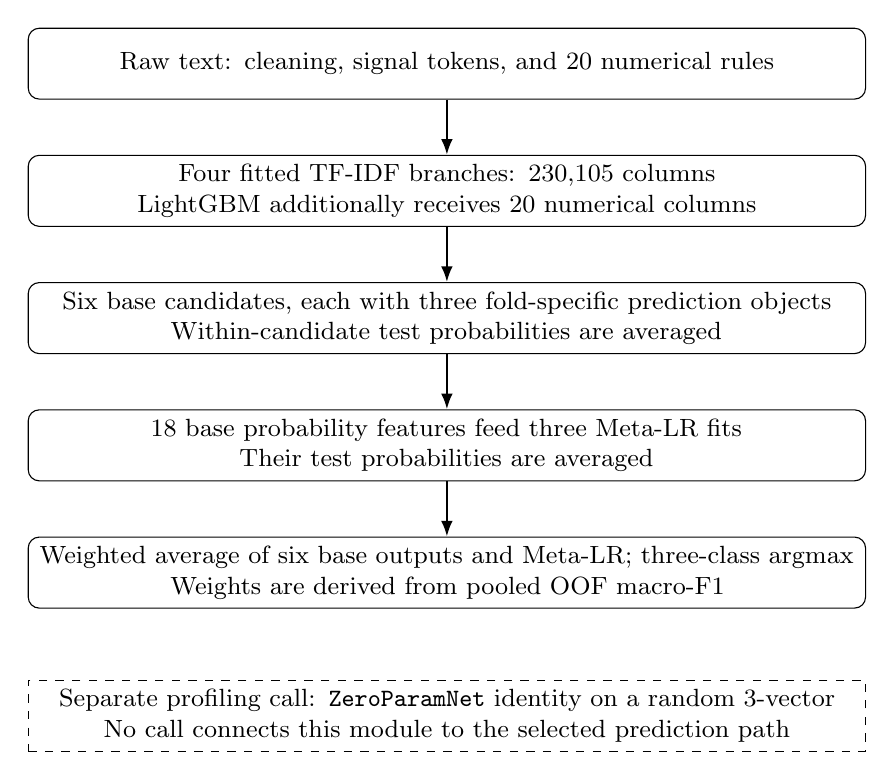
\begin{tikzpicture}[node distance=7mm, every node/.style={font=\small},
box/.style={draw,rounded corners,align=center,text width=10.4cm,minimum height=9mm},
arr/.style={-{Latex[length=2mm]},thick}]
\node[box] (text) {Raw text: cleaning, signal tokens, and 20 numerical rules};
\node[box,below=of text] (features) {Four fitted TF-IDF branches: 230,105 columns\\LightGBM additionally receives 20 numerical columns};
\node[box,below=of features] (base) {Six base candidates, each with three fold-specific prediction objects\\Within-candidate test probabilities are averaged};
\node[box,below=of base] (meta) {18 base probability features feed three Meta-LR fits\\Their test probabilities are averaged};
\node[box,below=of meta] (final) {Weighted average of six base outputs and Meta-LR; three-class argmax\\Weights are derived from pooled OOF macro-F1};
\draw[arr] (text)--(features);\draw[arr] (features)--(base);
\draw[arr] (base)--(meta);\draw[arr] (meta)--(final);
\node[draw,dashed,align=center,text width=10.4cm,below=9mm of final] {Separate profiling call: \texttt{ZeroParamNet} identity on a random 3-vector\\No call connects this module to the selected prediction path};
\end{tikzpicture}
\caption{Source-derived computation (S), not a measured deployment benchmark. Base outputs also enter the final weighted average directly, as specified in Equation~\ref{eq:ensemble}.}
\label{fig:pipeline}
\end{figure*}

\section{Recorded Results and Submission Provenance}
\label{sec:record}

\subsection{Candidate and Ensemble Results}
Table~\ref{tab:results} preserves printed candidate scores and fold values. LR\_C3 is the strongest base candidate. The weighted ensemble has pooled OOF macro-F1 0.5314, compared with 0.5306 for the simple average and 0.5221 for LR\_C3 (R). The rounded weighted-versus-base difference is 0.0093, or 0.93 percentage points (A). It is descriptive; the source selects weights, stopping points, and candidates using evaluation information, and no untouched comparison or paired prediction file is supplied.

\begin{table*}[t]
\small\centering
\caption{Recorded pooled and fold macro-F1 (R). Ensemble variants are scored on the same pooled OOF rows; no uncertainty interval is inferred from dependent folds.}
\label{tab:results}
\begin{tabular}{llrrrr}
\toprule
Candidate & Role & Pooled & Fold 1 & Fold 2 & Fold 3 \\
\midrule
LR\_C8 & Base & 0.5169 & 0.5158 & 0.5122 & 0.5227 \\
LR\_C3 & Base & 0.5221 & 0.5209 & 0.5171 & 0.5281 \\
SVC & Base & 0.4824 & 0.4860 & 0.4827 & 0.4782 \\
CNB & Base & 0.4391 & 0.4403 & 0.4356 & 0.4414 \\
SGD & Base & 0.4691 & 0.4675 & 0.4719 & 0.4678 \\
LightGBM & Base & 0.5160 & 0.5154 & 0.5136 & 0.5191 \\
Meta-LR & Stacker / ensemble member & 0.5218 & 0.5183 & 0.5169 & 0.5299 \\
\midrule
Weighted & Selected ensemble & 0.5314 & -- & -- & -- \\
Simple average & Alternative & 0.5306 & -- & -- & -- \\
Weighted + thresholds & Alternative & 0.5300 & -- & -- & -- \\
Average + thresholds & Alternative & 0.5287 & -- & -- & -- \\
\bottomrule
\end{tabular}
\end{table*}

Pooling computes F1 once from one prediction per training row. It is not the mean of fold F1 values because F1 is nonlinear in confusion counts. Nor does the OOF value directly evaluate the final test procedure: an OOF row uses fold-specific base outputs and its held-out meta fit, whereas test prediction averages three fits at both levels. The global OOF-derived weights add another difference between exclusion from a base fit and assessment of a frozen procedure.

The threshold search evaluates $30\times30=900$ pairs for each of the two ensemble probability arrays, adjusting classes 0 and 1 while leaving class 2's divisor at one (S). Its search interval is 0.1 to 0.9, omitting the unadjusted pair $(1,1)$. A lower best threshold score than the unadjusted score is therefore possible without a contradiction. The final source compares four variants and selects the unadjusted weighted ensemble. The displayed weighted thresholds 0.90, 0.87, and 1.00 are not on that selected prediction path.

\subsection{Confusion Counts and Error Structure}
Table~\ref{tab:confusion} transcribes the nine integer annotations in the updated notebook's embedded confusion figure. Row sums match the raw CSV supports and total 47,817. Reconstruction yields macro-F1 0.5314177985 and accuracy 0.5803166238 (A), consistent with the printed 0.5314. The three classwise values agree with the figure's four-decimal labels.

\begin{table*}[t]
\small\centering
\caption{Selected weighted-ensemble OOF confusion counts (R), with classwise metrics reconstructed from the displayed counts (A). Rows are actual labels; columns predicted labels.}
\label{tab:confusion}
\begin{tabular}{lrrrrrrr}
\toprule
Actual & Explicit & Subtle & Neutral & Support & Precision & Recall & F1 \\
\midrule
Explicit & 16,464 & 6,331 & 961 & 23,756 & 0.6501 & 0.6930 & 0.6709 \\
Subtle & 7,502 & 9,039 & 1,622 & 18,163 & 0.5118 & 0.4977 & 0.5046 \\
Neutral & 1,360 & 2,292 & 2,246 & 5,898 & 0.4651 & 0.3808 & 0.4188 \\
\midrule
Predicted & 25,326 & 17,662 & 4,829 & 47,817 & \multicolumn{3}{c}{Macro-F1 0.531418 (A)} \\
\bottomrule
\end{tabular}
\end{table*}

Neutral has the lowest F1 and recall. Of 4,829 examples predicted Neutral, 2,583 have a toxic label; 3,652 actual Neutral examples are assigned a toxic label. The largest off-diagonal count is 7,502 Subtle examples predicted Explicit. These are descriptions of disagreements, not explanations of sarcasm, lexical bias, or annotation error. Row level OOF predictions and paired candidate outputs are absent, so joint errors cannot be recovered. An always-Explicit predictor has arithmetic macro-F1 $2n_0/[3(n+n_0)]=0.221275$ (A), not a measured baseline experiment.

\subsection{Test Outputs and Version Mismatch}
The updated notebook prints 6,414 Explicit, 4,401 Subtle, and 1,140 Neutral test predictions, totaling 11,955 (R). It prints \texttt{parameters}=0.183 for its main export. Those generated CSVs were not supplied. The separately supplied \texttt{submission.csv} instead has 5,501, 4,139, and 2,315 predictions and constant NOP 39 (D). Its IDs match the three-class test and sample submission in order, but it is not the output described by the updated notebook. We preserve it as an earlier-version artifact and do not relabel it as the updated submission.

The updated source writes several files with different declared NOP values. Because zero equals the initial profiled value, its duplicate-skipping condition skips every zero-valued loop entry; the retained output confirms files for 0.1, 0.3, and 1, followed by the main file at 0.183. A later summary instructs submission of a zero-valued filename despite no corresponding save in this path. We distinguish invoked saves from report text. No save message establishes platform acceptance, compliance, or leaderboard rank.

\subsection{Timing and Retained State}
The recorded LR training sections take 2,601.7 and 2,625.0 seconds, and LightGBM takes 3,802.8 seconds (R). These three sections alone total 9,029.5 seconds, about 150.5 minutes (A), before other work. The notebook metadata reports about 152.4 minutes. Thus its concluding ``25--35 minutes'' claim is inconsistent with its retained timings. Those timings are historical output, not a newly controlled runtime benchmark, and no inference latency measurement is supplied.

LightGBM reports best iterations 149, 173, and 182 (R). No fitted vectorizers, base models, boosters, meta estimators, or OOF probability arrays are serialized by the inspected source. In-memory test arrays are generated before export, but the absence of saved model files prevents fresh-process raw-text replay. Historical environment uncertainty remains even though the source and recorded dimensions can now be inspected.

\section{Evaluation Validity}
\label{sec:validity}

\subsection{Global Representation and Label Statistics}
The recorded macro-F1 describes the notebook's retained development predictions. It does not show how a fully specified fitting and selection procedure performs on untouched examples. All four TF-IDF fits precede fold construction, so validation covariates affect vocabulary membership, frequency filtering, cap-based selection, and IDF. Hyperparameters can be fixed while the fitted representation still depends on evaluation text~\cite{kapoor2023leakage}.

Global class weights expose label statistics separately: $w_{I,c}=|I|/(3n_{I,c})$ includes every validation label in the class count used to fit a fold. LightGBM's fitting sample weights inherit the same dependency. The test text is transformed only, so this is an intra-training evaluation exposure, not evidence that the source fits vocabulary on unlabeled test text. Exact train/test text overlap is another dataset property, with a separate provenance from these code-level dependencies.

\subsection{Nonnested Meta-Training Dependencies}
For a meta learner $q^{(-a)}$ trained on $\{(z_i,y_i):i\notin V_a\}$ and evaluated on $V_a$, take a meta-training row $i\in V_b$, $b\ne a$. Its features came from base fits on $I\setminus V_b$, a set containing $V_a$. Thus
\begin{equation}
\begin{aligned}
y_{V_a}&\longrightarrow h_m^{(-b)}\longrightarrow z_i\\
&\longrightarrow\text{meta-training data}\longrightarrow q^{(-a)}.
\end{aligned}
\label{eq:path}
\end{equation}
A row in $V_a$ does receive base features from an estimator fit excluding $V_a$. However, the meta model evaluating that row was trained on other features whose construction used $y_{V_a}$. Row-level OOF exclusion therefore does not isolate the complete stacker. This structural dependency remains even if global preprocessing and class weights are provisionally accepted.

Rebuilding base OOF features only once for all meta folds preserves this path. It must instead be regenerated within the training partition of each outer assessment split, and again within the allowed fitting subset of each selection split. Equation~\ref{eq:path} establishes missing isolation, not the magnitude or direction of score distortion. Quantifying that would require a corrected rerun with protected assessment labels; none was performed here.

\subsection{Stopping, Weighting, and Candidate Selection}
LightGBM uses its validation labels for early stopping and subsequently reports macro-F1 on those same rows. The stopping objective is multiclass log loss; using a different reporting objective does not create a new evaluation sample. The ensemble weights are functions of pooled OOF F1 values, which are functions of all training labels. An OOF row's label can therefore influence its final weighted predictor through the aggregation weights even apart from meta-feature construction.

The two threshold searches each assess 900 choices on the entire pooled labeled OOF set. Their selected results and the unadjusted alternatives are then compared on those same labels. The final weighted result is selected from this development comparison. These repeated uses create opportunities for selection optimism~\cite{varma2006bias,cawley2010overfitting}; the audit measures no bias magnitude and does not attribute the rounded 0.0093 difference to any one component.

\subsection{Dependence and Uncertainty}
The three fitting subsets overlap: each pair shares roughly one-third of the full corpus, or half of either fitting subset. They are not independent repetitions. Stratification addresses class balance but does not protect against duplicates, shared authors, threads, or temporal dependence. Exact repetitions have been identified in the raw CSVs, but their allocation across the historical folds cannot be inspected from a saved fold-index file because none is provided.

There is no universally unbiased K-fold variance estimator based only on observed fold errors~\cite{bengio2004variance}. Paired comparisons also require retained row level predictions and a procedure appropriate to the data's independent units~\cite{dror2018significance}. We report neither a naive fold-based interval nor a significance claim. Such an interval would not resolve the fitting and selection exposures already traced.

\section{Parameter Boundaries and Score Provenance}
\label{sec:accounting}

\subsection{The Identity Module Is a Different Object}
The source defines \texttt{ZeroParamNet.forward(x)} to return $x$ unchanged. It has no trainable parameters. Profiling, when available, calls this module on a random three-element vector after the selected predictions already exist (S). No invocation applies the module to raw text, base probabilities, meta features, or selected outputs. Its zero count therefore describes a separate identity operation, not the harmful-content predictor.

The retained output prints \texttt{Manual NOP: 0} and \texttt{Final thop NOP: 0}, without the success line printed by the successful profiling branch. The variable is initialized to zero and remains zero when THOP is unavailable or fails. Consequently, the final printed zero alone cannot establish successful profiling. The source uses one positional input to this separate module, whereas the supplied competition description illustrates a two-input model call with token IDs and an attention mask. These interfaces do not determine a whole-system accounting boundary.

\subsection{Structural Inventory of the Selected Predictor}
The selected path contains six base candidates, each averaged over three fold-specific fits, plus three Meta-LR fits and seven combination weights. It also needs the cleaner, signals, four fitted vocabularies/IDF arrays, and LightGBM numerical rules. Unlike the earlier TinyLinear path, there is no learned PyTorch head in the updated predictor. Counting such a historical head would describe another version.

At recorded TF-IDF width $D=230{,}105$, each three-class multinomial LR fit has $3D$ coefficients and three intercepts. The two LR candidates each require three fits for their stored test averages. Meta-LR has 18 input probabilities and three output scores:
\begin{equation}
\begin{aligned}
N_{\mathrm{one\ base\ LR}}&=3D+3=690{,}318,\\
N_{\mathrm{six\ base\ LR}}&=6(3D+3)=4{,}141{,}908,\\
N_{\mathrm{three\ Meta\ LR}}&=3(3\times18+3)=171.
\end{aligned}
\label{eq:counts}
\end{equation}
These are arithmetic scalar inventories for specified matrices (A), not measured memory occupancy or a complete contest NOP. Coefficients for SVC and SGD, CNB state, calibrators, LightGBM trees, vocabularies, and IDF arrays remain outside this subtotal. Internal calibration can retain multiple fitted classifiers/functions per outer object; historical defaults and fitted internals are unknown~\cite{pedregosa2011scikit}.

No complete serialized artifact, peak RAM measurement, raw-text inference latency, or energy benchmark is available. Parameter counts, fitted state, serialized bytes, RAM, latency, and energy are distinct quantities~\cite{henderson2020systematic}. Averaging stored probability arrays is not a deployable substitute for the models needed to generate probabilities for unseen text. A resource comparison must apply the same declared boundary to every candidate.

\subsection{Fractional Export Values Are Not Measurements}
The main exported value rounds $F/2.9$ to three decimal places (S), producing 0.183 (R). It depends on a target score rather than on any model structure. A number of scalar parameters is a cardinality; 0.183, 0.1, and 0.3 are not measured counts. Zero is a valid count for the separate identity module, but it does not establish that a fitted ensemble has no state. No efficiency or compliance conclusion is supported by these exports.

With reconstructed $F=0.5314177984731835$ and $\epsilon=5\times10^{-16}$, the local ratio $F/(N+\epsilon)$ yields approximately $1.0628\times10^{15}$ at $N=0$ and 2.9039 at $N=0.183$ (A). These are arithmetic consequences of assigned denominators, not achieved leaderboard outcomes. The construction chooses a denominator near the desired ratio by design; it does not discover an efficient model.

\subsection{Authoritative Scoring Remains Unresolved}
The supplied details document presents $0.4F+0.6/[\log(N+1)+\epsilon]$ in its evaluation section, without specifying the log base, but later quotes $F/(N+\epsilon)$ in related-work notes. The original formula image and official scoring implementation are absent, and the pasted competition text omits the equation itself. The notebook implements the ratio for score projections; this is source evidence of a local formula, not verification of the competition contract.

The recorded figure combines earlier public values 0.24877, 0.25711, and 0.37286 with current OOF F1 0.5314 on an axis called ``Score / F1.'' These quantities have different provenance and do not form a verified generalization trajectory. An earlier private value 0.37500 is also unverified (X). Neither numerical proximity to a weighted formula nor a projected ratio authenticates leaderboard semantics. A definitive compliance statement requires the original parameter-count boundary and scorer; this audit alleges no organizer decision or verified competition violation.

\section{Corrected Prospective Protocol}
\label{sec:discussion}
The recorded ordering describes a development record, not a successful controlled ensemble experiment. The corrective protocol below is prospective (P); no listed training or benchmarking study was run by this audit. The artifact checks already performed should not be confused with these experiments.

First, freeze the dataset bytes, official label mapping, independent sampling units, and authorized use conditions. Inspect exact and near duplicates before splitting, and group or separate dependent posts where the intended evaluation requires it. Document prior exposure to the data. Hash inputs, record fold indices, and preserve the intended test IDs without importing the larger four-class data by filename alone.

Second, choose an outer assessment partition $E_a$ and training partition $T_a=I\setminus E_a$. Every data-dependent operation producing predictions on $E_a$ must use only $T_a$: vocabularies, IDF, class weights, base fitting, calibration, LightGBM stopping, meta fitting, ensemble weighting, threshold choice, and candidate selection. Base OOF features must be rebuilt within each permitted inner fitting subset rather than borrowed from a global OOF matrix. Stopping and selection need partitions within $T_a$; outer labels remain inaccessible until the complete predictor is frozen.

Third, compare standalone LR, a prespecified average, outcome-weighted averaging, and Meta-LR on identical allowed partitions, with stated tuning budgets. Each inference object must match the evaluated procedure: if deployment averages folds, assess that averaging procedure on untouched labels, rather than treating a row's single held-out fit as interchangeable. Save identifiers, true labels, probabilities, predictions, class ordering, and fold indices for valid paired analysis.

Fourth, tie additional experiments to the claims they would support. Marker-family and representation ablations are necessary for claims of feature benefit. Proper scores and reliability diagnostics are necessary for calibration claims. A permitted pretrained checkpoint on the same partitions is necessary for comparisons with transformers. Contextual error and subgroup studies, verified annotations, and an appropriate sampling frame are necessary for population or moderation claims. None follows from an aggregate OOF score alone.

Fifth, serialize and reload the complete raw-text prediction pipeline in a fresh process. Verify probability and label equivalence before reporting component sizes, total bytes, peak RAM, and latency with hardware, batch size, warmup, and repeated measurements~\cite{pineau2021reproducibility}. State training costs separately from inference. Store library versions, fitted calibration objects, LightGBM stopping points, and ensemble weights. Define any contest NOP according to its authoritative rules, and do not solve a score equation for a nominal count.

Finally, maintain a claim ledger linking each result to source operations, original outputs, measurement boundaries, and limitations. Keep the current notebook, older submissions, and archived drafts distinguishable. A source correction, a successful CSV save, a portal receipt, and a leaderboard measurement are separate evidence events.

\section{Limitations and Responsible Interpretation}
\label{sec:limitations}
The updated source and retained outputs are inspectable, and the supplied CSVs agree with its printed supports. However, no hash recorded during the historical run establishes that those exact bytes were used. The audit does not rerun training, recover missing OOF rows, inspect fitted model states, or verify a platform submission. Unknown package versions and contradictory device metadata limit replay. Exact-string duplication is checked; semantic duplicates and shared-user/thread structure are not.

The threats are distinct: internal, because fitting and selection use evaluation information; external, because one record does not establish a population claim; construct-related, because label definitions lack a complete annotation manual; statistical, because folds and selection outcomes are dependent; and measurement-related, because the counted identity object differs from the selected predictor. Neither the direction of score distortion nor deployment cost is measured.

The three-way argmax is a research prediction, not a moderation policy. Substring matching can activate inside benign words, and identity-related cues do not model whether a speaker endorses, condemns, quotes, or reclaims an expression~\cite{blodgett2020language,rottger2021hatecheck}. No operating threshold, contextual safety, appeal process, or deployment benefit has been established. No legal basis, consent, ethics approval, or independent redistribution permission is inferred from public-source collection or from a supplied license description.

\section{Conclusion}
\label{sec:conclusion}
This case study reconstructs the updated LightBanglaHC record: 47,817 training rows, four fitted TF-IDF branches, six base candidates, a Meta-LR component, and a selected weighted ensemble. Its reconstructed macro-F1 0.531418 agrees with the notebook's 0.5314; the rounded comparison with LR\_C3 at 0.5221 remains descriptive. The original five-fold TinyLinear numbers and supplied NOP-39 CSV belong to other versions and cannot verify this execution.

Three findings transfer. Row-level OOF exclusion does not isolate a full procedure when evaluation labels remain ancestors of meta-training features, stopping choices, or combination weights. A zero-parameter identity operation does not account for the fitted state that produces harmful-content predictions. A fractional denominator selected to achieve a desired score is not a parameter measurement. Every predictive or efficiency claim should name its inference object, fitting and selection ancestry, accounting boundary, and supporting evidence. This remains an inspectable methodological case, not a validated deployment system.

\subsubsection*{Disclosure of Interests.}
Funding, competing interests, ethics review or exemption, data permissions, and annotator-welfare information were not supplied with the inspected artifacts. This is not a declaration of no funding or no interests; authors must finalize applicable disclosures before submission. This revision used AI-assisted literature organization, drafting, source inspection, arithmetic checking, and typesetting. It produced no new training results and authorized no data use.

\bibliographystyle{ijcvsplatex-num}
\bibliography{references}
\end{document}
